\documentclass[tikz,border=8pt]{standalone}
\usepackage{amsmath,amssymb}
\usetikzlibrary{arrows.meta,automata,positioning,quotes}
\begin{document}
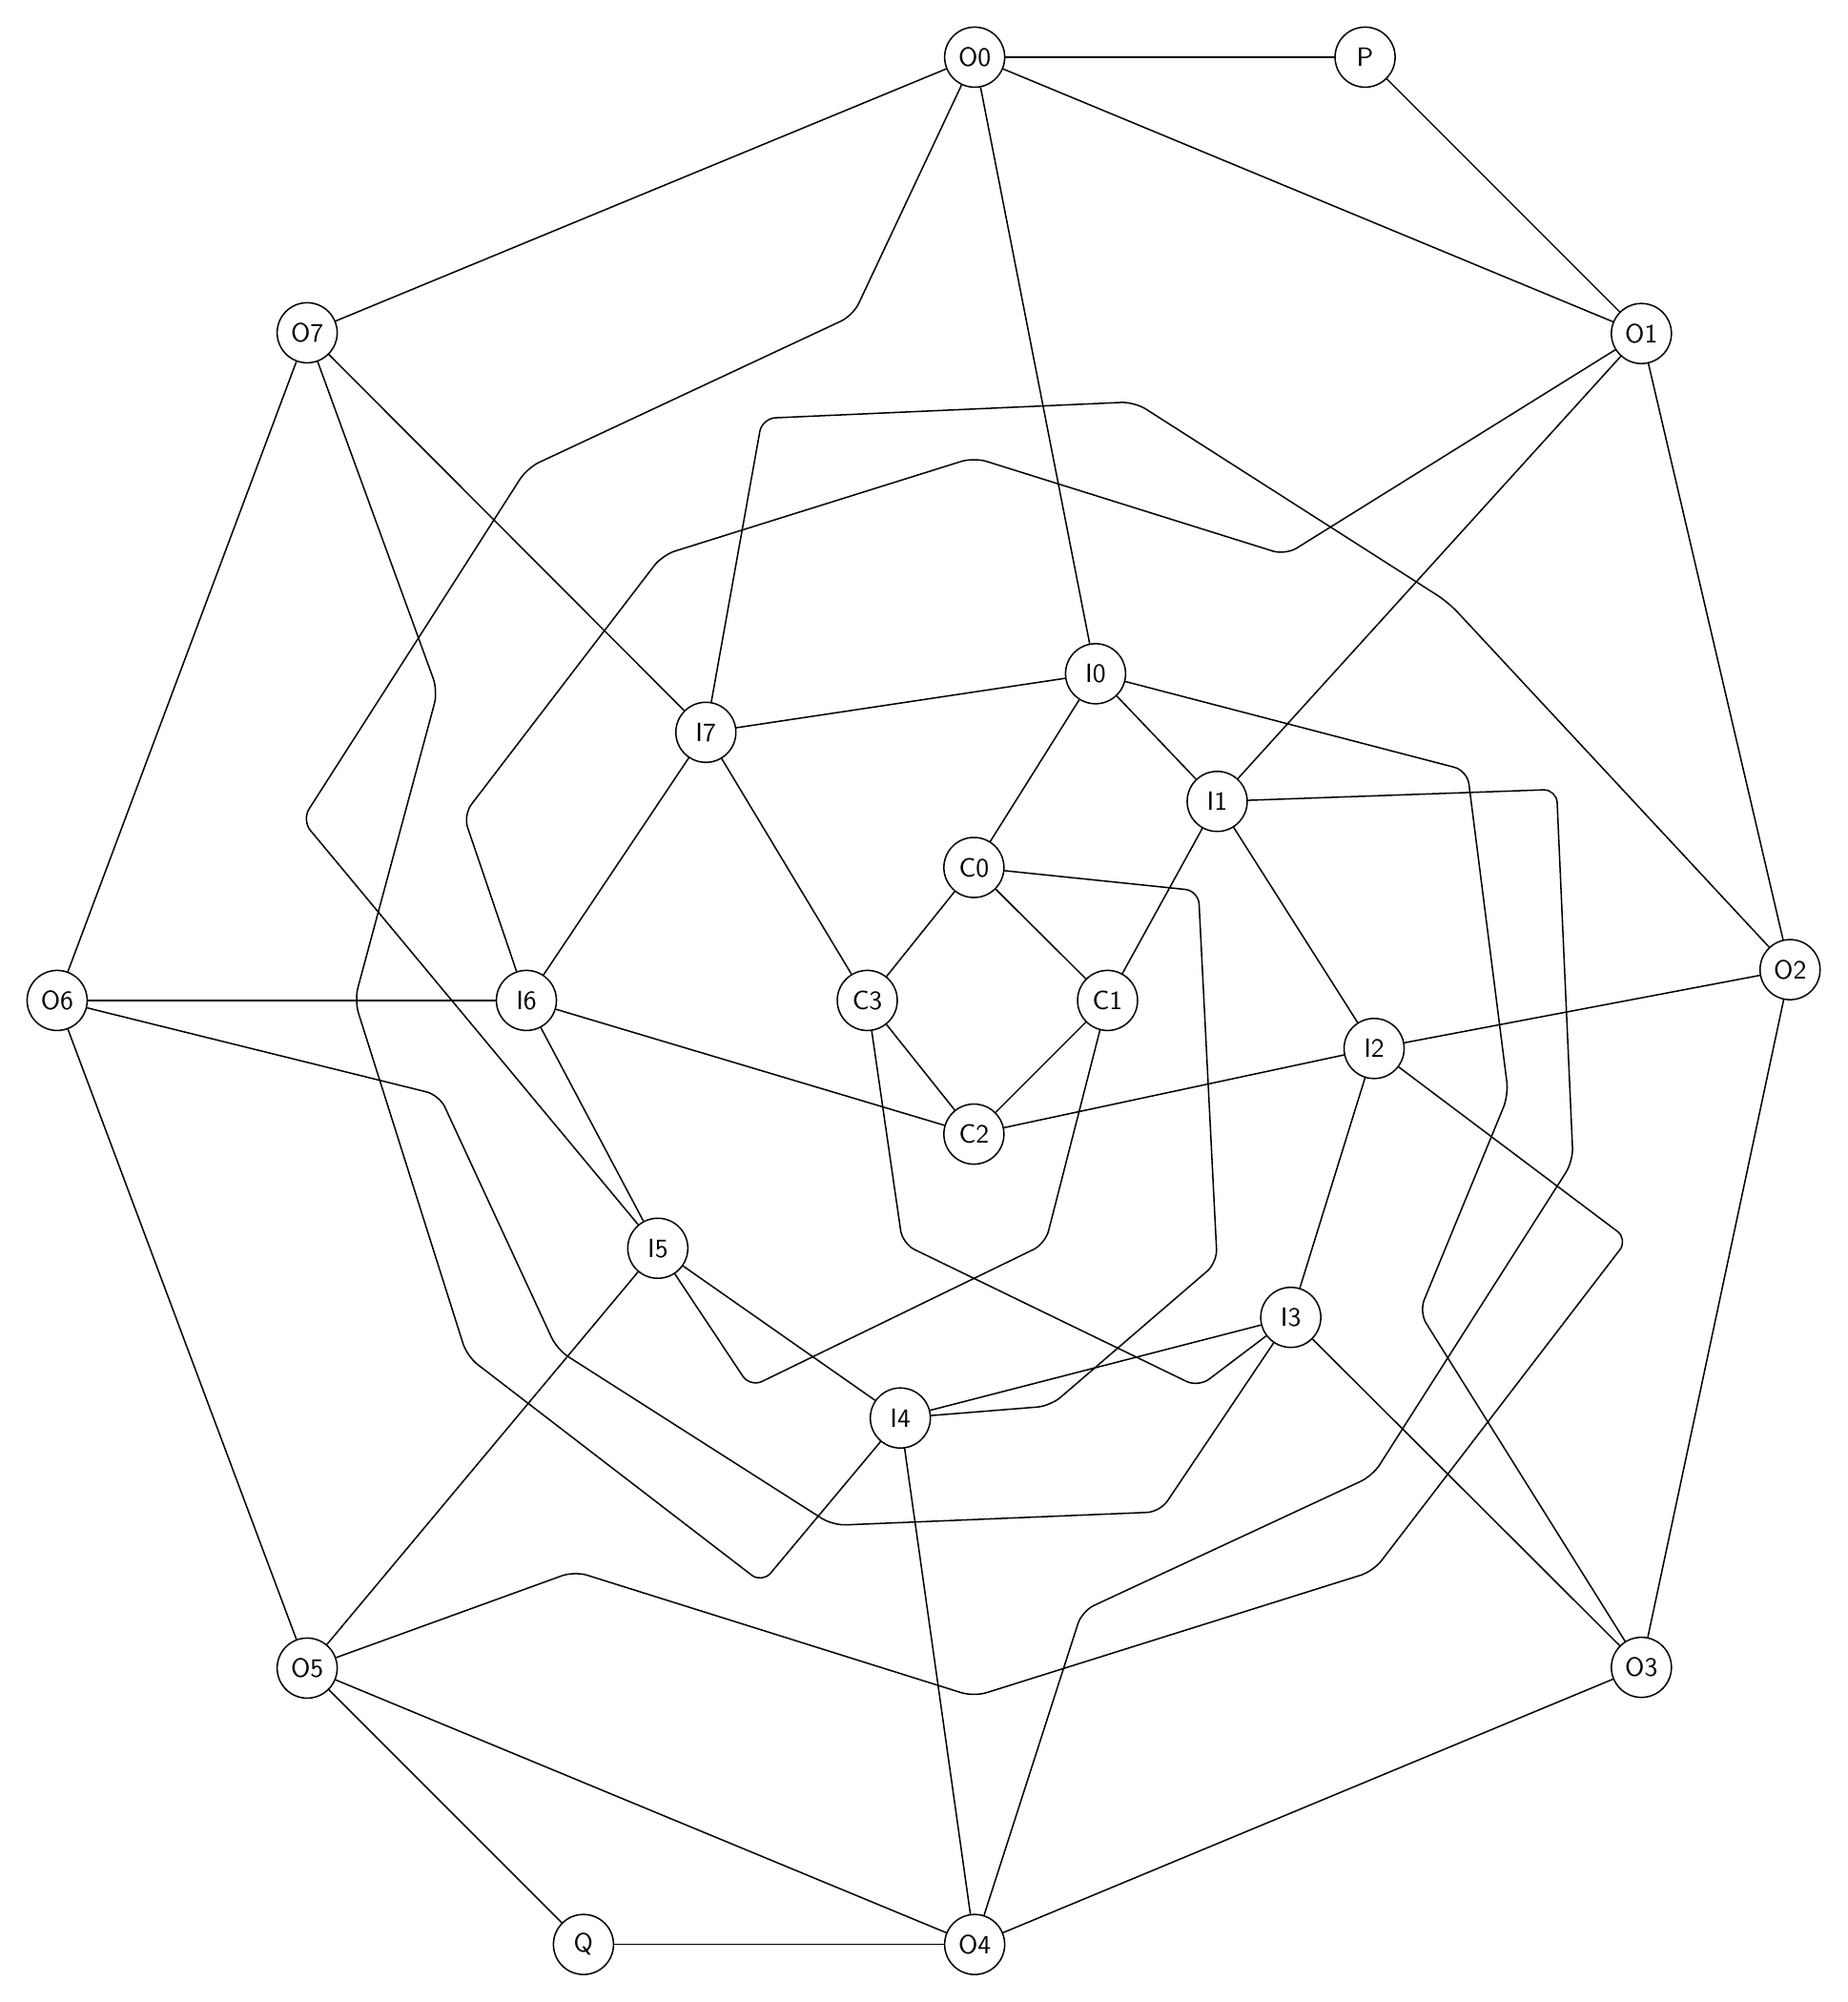
\begin{tikzpicture}[x=1cm,y=1cm]
\tikzset{
  graphnode/.style={circle,draw=black,line width=0.55pt,minimum size=8mm,inner sep=1pt,font=\sffamily},
  graphedge/.style={draw=black,line width=0.55pt,line cap=round,line join=round},
  directed/.style={graphedge,-{Stealth[length=2.4mm,width=2.0mm]}},
  undirected/.style={graphedge}
}
\node[graphnode] (n_O0) at (0.02,12.59) {O0};
\node[graphnode] (n_O1) at (8.90,8.91) {O1};
\node[graphnode] (n_O2) at (10.88,0.44) {O2};
\node[graphnode] (n_O3) at (8.90,-8.85) {O3};
\node[graphnode] (n_O4) at (0.02,-12.54) {O4};
\node[graphnode] (n_O5) at (-8.87,-8.86) {O5};
\node[graphnode] (n_O6) at (-12.20,0.03) {O6};
\node[graphnode] (n_O7) at (-8.87,8.92) {O7};
\node[graphnode] (n_I0) at (1.63,4.38) {I0};
\node[graphnode] (n_I1) at (3.25,2.68) {I1};
\node[graphnode] (n_I2) at (5.34,-0.61) {I2};
\node[graphnode] (n_I3) at (4.23,-4.19) {I3};
\node[graphnode] (n_I4) at (-0.97,-5.53) {I4};
\node[graphnode] (n_I5) at (-4.20,-3.27) {I5};
\node[graphnode] (n_I6) at (-5.95,0.03) {I6};
\node[graphnode] (n_I7) at (-3.56,3.60) {I7};
\node[graphnode] (n_C0) at (0.01,1.80) {C0};
\node[graphnode] (n_C1) at (1.79,0.03) {C1};
\node[graphnode] (n_C2) at (0.01,-1.75) {C2};
\node[graphnode] (n_C3) at (-1.41,0.03) {C3};
\node[graphnode] (n_P) at (5.22,12.59) {P};
\node[graphnode] (n_Q) at (-5.19,-12.54) {Q};
\draw[undirected] (n_O0) -- (n_O1);
\draw[undirected] (n_O1) -- (n_O2);
\draw[undirected] (n_O2) -- (n_O3);
\draw[undirected] (n_O3) -- (n_O4);
\draw[undirected] (n_O4) -- (n_O5);
\draw[undirected] (n_O5) -- (n_O6);
\draw[undirected] (n_O6) -- (n_O7);
\draw[undirected] (n_O7) -- (n_O0);
\draw[undirected] (n_I0) -- (n_I1);
\draw[undirected] (n_I1) -- (n_I2);
\draw[undirected] (n_I2) -- (n_I3);
\draw[undirected] (n_I3) -- (n_I4);
\draw[undirected] (n_I4) -- (n_I5);
\draw[undirected] (n_I5) -- (n_I6);
\draw[undirected] (n_I6) -- (n_I7);
\draw[undirected] (n_I7) -- (n_I0);
\draw[undirected] (n_O0) -- (n_I0);
\draw[undirected] (n_O1) -- (n_I1);
\draw[undirected] (n_O2) -- (n_I2);
\draw[undirected] (n_O3) -- (n_I3);
\draw[undirected] (n_O4) -- (n_I4);
\draw[undirected] (n_O5) -- (n_I5);
\draw[undirected] (n_O6) -- (n_I6);
\draw[undirected] (n_O7) -- (n_I7);
\draw[undirected,rounded corners=5pt] (n_I0) -- (6.58,3.09) -- (7.13,-1.23) -- (5.94,-4.12) -- (n_O3);
\draw[undirected,rounded corners=5pt] (n_I1) -- (7.77,2.84) -- (7.99,-2.11) -- (5.32,-6.30) -- (1.45,-8.10) -- (n_O4);
\draw[undirected,rounded corners=5pt] (n_I2) -- (8.72,-3.15) -- (5.33,-7.57) -- (0.01,-9.24) -- (-5.31,-7.57) -- (n_O5);
\draw[undirected,rounded corners=5pt] (n_I3) -- (2.49,-6.78) -- (-1.87,-6.96) -- (-5.54,-4.62) -- (-7.11,-1.23) -- (n_O6);
\draw[undirected,rounded corners=5pt] (n_I4) -- (-2.81,-7.73) -- (-6.74,-4.71) -- (-8.24,0.03) -- (-7.13,4.15) -- (n_O7);
\draw[undirected,rounded corners=5pt] (n_I5) -- (-8.94,2.43) -- (-5.94,7.12) -- (-1.60,9.15) -- (n_O0);
\draw[undirected,rounded corners=5pt] (n_I6) -- (-6.79,2.50) -- (-4.14,5.96) -- (0.01,7.26) -- (4.16,5.96) -- (n_O1);
\draw[undirected,rounded corners=5pt] (n_I7) -- (-2.81,7.78) -- (2.15,8.00) -- (6.33,5.33) -- (n_O2);
\draw[undirected] (n_C0) -- (n_C1);
\draw[undirected] (n_C1) -- (n_C2);
\draw[undirected] (n_C2) -- (n_C3);
\draw[undirected] (n_C3) -- (n_C0);
\draw[undirected] (n_C0) -- (n_I0);
\draw[undirected,rounded corners=5pt] (n_C0) -- (3.00,1.49) -- (3.25,-3.46) -- (1.03,-5.37) -- (n_I4);
\draw[undirected] (n_C1) -- (n_I1);
\draw[undirected,rounded corners=5pt] (n_C1) -- (0.96,-3.21) -- (-2.97,-5.12) -- (n_I5);
\draw[undirected] (n_C2) -- (n_I2);
\draw[undirected] (n_C2) -- (n_I6);
\draw[undirected,rounded corners=5pt] (n_C3) -- (-0.94,-3.21) -- (3.00,-5.12) -- (n_I3);
\draw[undirected] (n_C3) -- (n_I7);
\draw[undirected] (n_P) -- (n_O0);
\draw[undirected] (n_P) -- (n_O1);
\draw[undirected] (n_Q) -- (n_O4);
\draw[undirected] (n_Q) -- (n_O5);
\end{tikzpicture}
\end{document}
